% !TEX TS-program = pdflatex
%\RequirePackage{lineno}
\documentclass[aps,prc,twocolumn,floatfix,showpacs,preprintnumbers,amsmath,amssymb,superscriptaddress]{revtex4-1}
\usepackage{hyperref}
\usepackage{latexsym}
\usepackage{verbatim}
\usepackage{graphics}
\usepackage{caption}
\usepackage{subfigure}
\usepackage{amsmath}
\captionsetup{justification=centerlast,font=small,margin=0.5cm}
\usepackage{setspace}
\usepackage{graphicx,amsmath,color}% Include figure files
\usepackage[normalem]{ulem} %for strikeouts
\usepackage{todonotes}
\usepackage{placeins}

\providecommand{\Journal}[4] {#1 {\bf #2}, #3 (#4)}
\providecommand{\EPJC}{Eur. Phys. J. C }
\providecommand{\NCA}{Nuovo Cimento }
\providecommand{\NIM}{Nucl. Instr. Methods }
\providecommand{\NIMA}{Nucl. Instr. Meth. A }
\providecommand{\NPA}{Nucl. Phys. A }
\providecommand{\NPB}{Nucl. Phys. B }
\providecommand{\NHPA}{Nucl. Hadr. Phys. A }
\providecommand{\PLB}{Phys. Lett. B }
\providecommand{\PR}{Phys. Rev. }
\providecommand{\PRL}{Phys. Rev. Lett. }
\providecommand{\PRC}{Phys. Rev. C }
\providecommand{\PRD}{Phys. Rev. D }
\providecommand{\RMP}{Rev. Mod. Phys. }
\providecommand{\ZPC}{Z. Phys. C }
\providecommand{\qqb}{$q\bar{q}$~}
\newcommand{\bff}{{}}

\definecolor{lightred}{rgb}{1,0.5,0.5}
\definecolor{lightgreen}{rgb}{0.5,1,0.5}
\definecolor{darkgreen}{rgb}{0.5,0.9,0.5}

\def\piz{\pi^{0}}
\def\pizT{$\pi^{0} \ $}
\def\epemT{$ e^+e^-  $}
\def\epem{e^+e^-}
\begin{document}
\preprint{}


\title{Photoproduction of $\pi^0$ on Hydrogen Target with CLAS}

%To be submitted to Phys. Rev. Lett.\\
%\bf -- DRAFT -- VERSION 1.1\\
%\bf \today}

\newcommand*{\ODU}{Old Dominion University, Norfolk, VA 23529, USA}
%1   Institut f¨ur Kernphysik, Forschungszentrum J¨ulich 52424, J¨ulich, Germany

%2   Institut fu¨r Experimentalphysik I, Ruhr–Universita¨t Bochum, Universita¨tsstr. 150, 44780 Bochum, Germany

%3  JARA–FAME, Ju¨lich Aachen Research Alliance, Forschungszentrum Ju¨lich, 52425 Ju¨lich, and RWTH Aachen, 52056 Aachen, Germany
\newcommand*{\IKP}{Institut f\"ur Kernphysik, Forschungszentrum J\"ulich, 52424 J\"ulich, Germany}
\newcommand*{\BOCHUM}{Institut f\"ur Experimentalphysik I, Ruhr–Universit\"at Bochum, Universit\"atsstr. 150, 44780 Bochum, Germany}
\newcommand*{\JARA}{ JARA–FAME, J\"ulich Aachen Research Alliance, Forschungszentrum J\"ulich, 52425 J\"ulich, and RWTH Aachen, 52056 Aachen, Germany}
\newcommand*{\PNPI}{Petersburg Nuclear Physics
	Institute, Gatchina, St.\ Petersburg 188300, Russia}
\newcommand*{\KYUNGPOOK} {Kyungpook National University, 702-701, Daegu, 
	Republic of Korea}
\newcommand*{\INR}{Institute for Nuclear Research, 117312, Moscow, Russia}
\newcommand*{\CUA}{Catholic University of America, Washington, DC 20064} 
\newcommand*{\JLAB}{Thomas Jefferson National Accelerator Facility, Newport 
	News, VA 23606}
\newcommand*{\UVA}{University of Virginia, Charlottesville, VA 22904, USA}
\newcommand*{\CMU}{Carnegie Mellon University, Pittsburg, PA 15213, USA}

\newcommand*{\ANL}{Argonne National Laboratory, Argonne, IL 60439, USA}
\newcommand*{\ASU}{Arizona State University, Tempe, AZ 85287, USA}
\newcommand*{\CSUDH}{California State University, Dominguez Hills, Carson, 
	CA 90747, USA}
\newcommand*{\CANISIUS}{Canisius College, Buffalo, NY, USA}
\newcommand*{\SACLAY}{CEA, Centre de Saclay, Irfu/Service de Physique 
	Nucl\'eaire, 91191 Gif-sur-Yvette, France}
\newcommand*{\CNU}{Christopher Newport University, Newport News, VA 23606, 
	USA}
\newcommand*{\UCONN}{University of Connecticut, Storrs, CO 06269, USA}
\newcommand*{\EDINBURGH}{University of Edinburgh, Edinburgh EH9 3JZ, United 
	Kingdom}
\newcommand*{\FU}{Fairfield University, Fairfield, CT 06824, USA}
\newcommand*{\FIU}{Florida International University, Miami, FL 33199, USA}
\newcommand*{\FSU}{Florida State University, Tallahassee, FL 32306, USA}
\newcommand*{\GWU}{The George Washington University, Washington, DC 20052, USA}
\newcommand*{\ISU}{Idaho State University, Pocatello, Idaho 83209, USA}
\newcommand*{\INFNFE}{INFN, Sezione di Ferrara, 44100 Ferrara, Italy}
\newcommand*{\INFNFR}{INFN, Laboratori Nazionali di Frascati, 00044 Frascati, 
	Italy}
\newcommand*{\INFNGE}{INFN, Sezione di Genova, 16146 Genova, Italy}
\newcommand*{\INFNRO}{INFN, Sezione di Roma Tor Vergata, 00133 Rome, Italy}
\newcommand*{\ORSAY}{Institut de Physique Nucl\'eaire ORSAY, Orsay, France}
\newcommand*{\ITEP}{Institute of Theoretical and Experimental Physics, Moscow, 
	117259, Russia}
\newcommand*{\JMU}{James Madison University, Harrisonburg, VA 22807, USA}
\newcommand*{\KNU}{Kyungpook National University, Daegu 702-701, Republic of 
	Korea}
\newcommand*{\LPSC}{LPSC, Universite Joseph Fourier, CNRS/IN2P3, INPG, Grenoble, 
	France

}
\newcommand*{\UNH}{University of New Hampshire, Durham, New Hampshire 03824, 
	USA}
\newcommand*{\NSU}{Norfolk State University, Norfolk, VA 23504, USA}
\newcommand*{\OHIOU}{Ohio University, Athens, Ohio  45701, USA}
\newcommand*{\RPI}{Rensselaer Polytechnic Institute, Troy, NY 12180, USA}
\newcommand*{\ROMAII}{Universita' di Roma Tor Vergata, 00133 Rome Italy}
\newcommand*{\MSU}{Skobeltsyn Nuclear Physics Institute, 119899 Moscow, Russia}
\newcommand*{\SCAROLINA}{University of South Carolina, Columbia, South Carolina 
	29208, USA}
\newcommand*{\UNIONC}{Union College, Schenectady, NY 12308}
\newcommand*{\UTFSM}{Universidad T\'{e}cnica Federico Santa Mar\'{i}a, Casilla 
	110-V Valpara\'{i}so, Chile}
\newcommand*{\GLASGOW}{University of Glasgow, Glasgow G12 8QQ, United Kingdom}
\newcommand*{\VIRGINIA}{University of Virginia, Charlottesville, VA 22901, 
	USA}
\newcommand*{\WM}{College of William and Mary, Williamsburg, VA 23187, USA}
\newcommand*{\YEREVAN}{Yerevan Physics Institute, 375036 Yerevan, Armenia}
\newcommand*{\NOWCNU}{Christopher Newport University, Newport News, VA
	23606, USA}
\newcommand*{\NOWLANL}{Los Alamos National Laboratory, Los Alamos, NM 87544, 
	USA}
\newcommand*{\NOWMSU}{Skobeltsyn Nuclear Physics Institute, 119899 Moscow, 
	Russia}
\newcommand*{\NOWORSAY}{Institut de Physique Nucl\'eaire ORSAY, Orsay, France}
\newcommand*{\TUFTS}{Tufts University, Medford, MA 02155, USA}
 %%%%%%%%%%%%%%% END OF Latex Macros for institute addresses  %%%%%%%%%%%%%%%%%%%%%%

\author {Michael~C.~Kunkel}
\altaffiliation[Now at the ]{Institut f\"ur Kernphysik, Forschungszentrum J\"ulich, 52424 J\"ulich, Germany}%Lines break automatically or can be forced with \\
\affiliation{\ODU}
\author {Moskov~J.~Amaryan}
\thanks{Corresponding author; mamaryan@odu.edu}
%\email{mamaryan@odu.edu}
\affiliation{\ODU}
\author {Igor~I.~Strakovsky}
\affiliation{\GWU}
\author {James~Ritman}
\affiliation{\IKP}
\affiliation{\BOCHUM}
\author{Gary~R.~Goldstein}
\affiliation{\TUFTS}
%%%%%%%%%%%%%%%%%%%%%%%%%%%%%%%%%%%%%%%%%%%%%%%%%%%%%%%%%%%%%%%%%%%%%%%%%%%%
%
\vskip 1.50in
\vskip 2in

%---------------------------------------------
\begin{abstract}
\centerline{\Large Abstract}
\vskip 0.2in
We report the first high precision measurement of exclusive $\pi^0$ 
photoproduction cross section in Dalitz decay and conversion mode on a 
hydrogen target in a wide kinematic range with the CLAS 
setup at Thomas Jefferson National Accelerator Facility. 
Measurement is performed in the reaction $\gamma p\to 
pe^+e^-X(\gamma)$ using a tagged photon beam spanning an 
energy interval from the ``resonance'' to the ``Regge'' regimes, i.e photon energies
$E = 1.25-5.55$~GeV. The final state particles particles $p;e^+;e^-$ 
are detected while the photon is not detected. The $\pi^0$ is 
identified by analyzing the missing mass of proton.  This new data quadrupled 
the world bremsstrahlung database above E = 2~GeV. Our 
data appear to favor the Regge pole model and the quark 
counting rule while disfavoring the Handbag model.
\end{abstract}
%---------------------------------------------

\pacs{12.38.Aw, 13.60.Rj, 14.20.-c, 25.20.Lj}
\maketitle

%---------------------------------------------
%\textbf{Introduction:} 
%In elementary particle physics involving 
%energies less than 2.5~GeV in the c.m. total energy $W$ 
%("resonance" regime), the study of lightest meson 
%($\pi^0$ and 
%$\eta$) photoproduction has always been a complementary tool to 
%elastic $\pi$N scattering. 
%The complications introduced by the 
%spin 1 of the photon was a matter of algebra rather than 
%a matter of dynamics; this is not the case in the high-energy 
%domain. Because photoproduction involves three kind of different 
%masses and because the spin of particles is high enough, one 
%encounters both the problem of daughter trajectories and of 
%conspiracy relations. Therefore, this process and the associated 
%one of vector meson production are really very interesting at 
%the present. The possibility that the scattering amplitude for 
%photoproduction might be reggeized has not been cast in doubt 
%as Ader, Capdeville, and Salin noticed~\cite{Ader}.  
%This experiment is a unique opportunity to bridge resonance and 
%high-energy, in particular, "Regge", regimes and increases 
%available database above resonance range by significant amount.
%---------- Possible replacement of Intro -----
%The spectrum of the baryons has been a subject of intense experimental and theoretical work since the discovery of the $\pi+N$ $\Delta$ resonance by Anderson and Fermi~\cite{Fermi}. 
The rich $\pi + N$ resonance spectrum for center-of-mass (c.m.) energies up to 2.5~GeV provides insights and challenges concerning the workings of the strong interaction through partial wave expansions, exchange potentials, non-relativistic quark models and QCD. The $\pi^0$ and 
$\eta$ photoproduction has always been a complementary tool to investigate and constrain 
%elastic $\pi$N scattering. 
%other channels that access the nucleon resonances - $\pi$ photoproduction, electroproduction and neutrino production - constrain 
the various models and lead to further insights. At the interface between the crowded low energy resonance cross section and the smooth higher energy behavior, traditionally described by Regge poles~\cite{Ader}, lies a region in which hadronic duality provides an interpolation description of the cross section behavior. Exclusive $\pi$ photoproduction and $\pi$ nucleon elastic scattering show this duality in a semi-local sense through Finite Energy Sum Rules (FESR)~\cite{Armenian}. The connection to QCD is more tenuous for on-shell photoproduction of pions at small scattering angles, but the quark content can become manifest through fixed angle dimensional counting rules~\cite{Stan} as well as being evident in semi-inclusive or exclusive electroproduction of pions, described through Transverse Momentum Distributions (TMDs)  and Generalized Parton Distributions (GPDs).
% through large virtual photon exchanges, underpinned by the parton distributions, the TMDs and GPDs. How to interpret the gap between real $Q^2=0$ photoproduction of $\pi$'s and $\eta$'s and the virtual $\pi$ and $\eta$ production for $Q^2 \gg \Lambda_{QCD}^2$ is an open question. 
%What is well known, since the Kroll-Ruderman theorem~\cite{K-R}, is the role that pion photoproduction plays in constraining the $\pi + N$ resonances, in the resonance region and above.

This experiment is a unique opportunity to bridge resonance and 
high-energy, in particular, ``Regge", regimes and increases the
available database above the resonance range by a significant amount.




%---------------------------------------------------
%\textbf{Regge Pole Model:} 
The Regge pole description of photoproduction amplitudes relies on 
already known Regge 
trajectories and coupling constants. The unitary cut amplitudes in meson
%count on the independent description of the elementary 
photoproduction are interpreted as rescattering of on-shell meson-nucleon amplitudes.  
%This approach is "parameter free". There is little degrees of 
%freedom left. One possibility is the relative sign between 
%amplitudes. 
The phases between the poles and the elastic neutral 
pion re-scattering 
%is fixed by unitarity 
%(for the absorptive part and consequently for the real part), 
%and that phases 
are critical in determining the polarizations and the constructive or destructive interferences that appear in the resonance spectrum.
% relative 
%phase of the amplitudes in the inelastic cuts is not 
%determined by the cross section of the corresponding elementary 
%reactions. A second possibility is a more accurate description 
%of these elementary cross sections, but this is second order.  

The Regge pole and cut model for higher energies above the
resonance regime for $\pi^0$ and $\eta$ photoproduction developed by Goldstein 
and Owens~\cite{Goldstein} has the exchange of leading Regge 
trajectories with appropriate t-channel quantum numbers along 
with Regge cuts generated via 
%initial or 
final state rescattering 
through Pomeron exchange. There are two allowed t-channel J$^{PC}$ 
quantum numbers series, the odd-signature 1$^{--}$ and the 1$^{+-}$, 
corresponding to the $\rho^0$, $\omega$, and the $b^0_1$, $h_1$ 
Reggeons, respectively. The Regge couplings to the nucleon were fixed by 
reference to electromagnetic form factors, SU(3)$_{flavor}$, and low 
energy nucleon-nucleon meson exchange potentials.  The Primakoff 
effect is not included in the parameterization.  Similar approaches 
to some extent were developed by Laget~\cite{Laget}, Mathieu, 
Fox, and Szczepaniak~\cite{Mathieu}, and recently, Donnachie and 
Kalashnikova~\cite{Donnachie}.  
The model of Laget is presumably 
%Two Regge models are 
valid within the full angular range ($\theta = 
0^\circ - 180^\circ$)~\cite{Laget} while the others are 
good for different ranges of the forward direction (from $|t| = 
-t_{min}$ at $\theta=0$ to $\theta=\pi/2$)
%0 - 1$~GeV$^2$)
~\cite{Goldstein,Mathieu,Donnachie}. Here, we examine
how Regge phenomenology works for the full CLAS energy range, i.e.
E $>$ 2.8~GeV.

%--------------------------------------------------
%\textbf{Handbag Model:} 
The introduction of the handbag mechanism, 
developed by Kroll \textit{et al.}~\cite{Kroll}, has provided 
complimentary possibilities for the interpretation of hard 
exclusive reactions. In this approach, the reaction is factorized 
into two parts, one quark from the incoming and one from the 
outgoing nucleon participate in the hard sub-process, which is 
calculable using pQCD. The soft part consists of all the 
other partons that are spectators and can be described in 
terms of GPDs~\cite{HM}. The handbag model applicability 
requires a hard scale, which, for meson photoproduction, is only 
provided by large transverse momentum. That corresponds to large 
angle production, roughly
for $-0.6~\leq\cos\theta~\leq 0.6$.  Here, we examined how 
the handbag model may extend for the $\gamma p\to p\pi^0$ 
case as Kroll \textit{et al.} proposed.  
%This approach was developed to understand the nature of the observation which the HERMES Collaboration made~\cite{Moskov}.
%--------------------------------------------------
%\textbf{Scaling:} 
Binary reactions in QCD, with large momentum 
transfer occur via 
gluon and quark exchanges between colliding particles. The 
quark counting rule of Brodsky and 
Farrar~\cite{Stan} has a simple recipe to predict the energy 
dependence of the differential cross sections of two-body
reactions at large angles when $t/s$ is finite and is kept 
constant.  The lightest meson photoproduction was examined 
in terms of the counting rule~\cite{Anderson,Jenkins,Zhu,
Chen,Kong}. As has been observed, first of all at SLAC by 
Anderson \textit{et al.}, the reaction $\gamma p\to\pi^+n$ 
shows agreement with constituent counting rules that predict 
the cross section should vary as $s^{-7}$~\cite{Anderson}. 
The agreement extends down to s = 6~GeV$^2$ where baryon 
resonances are still playing a role.  Here, we examined how
the counting rule is applicable to the $\gamma p\to\pi^0p$ 
up to s = 10~GeV$^2$.

Previous bremsstrahlung measurements for $2~\leq E\leq 
18$~GeV (1964 -- 1979) gave 451 data points $d\sigma/dt(|t|)$s for 
$\gamma p\to p\pi^0$~\cite{brem}.  Existing bremsstrahlung 
world data on photoproduction of neutral pions on proton 
target have very large systematic uncertainties and do not 
have sufficient accuracy to perform comprehensive 
phenomenological analyses.  
%While 
The recent tagged CLAS $g1c$ 
measurement has overall systematic uncertainty of 5\% and 
its contribution for $2~\leq E\leq 2.9$~GeV is limited by 
164 $d\sigma/dt(|t|)$s~\cite{du07}.  

In this work, we provide a large set of cross sections from 
E = 1.275--5.425~MeV in laboratory photon energy, 
corresponding to a c.m. energy $W$ range of 1.81--3.33~GeV.  
We have, therefore, tried to 
%confront 
compare the Regge pole, the
handbag, and the quark counting rule phenomenology with the 
new CLAS experimental information on the $d\sigma/dt(|t|)$ 
for the $\gamma p\to\pi^0p$ above the "resonance" regime. As will 
be seen, this data set (it quadrupled the world bremsstrahlung 
database above E = 2~GeV) and previous CLAS $g1c$ tagged 
measurements greatly constrain the high energy phenomenology.

%\textbf{Experiment:} 
The experiment is performed with the CLAS setup 
at TJNAF using a tagged photon beam produced by bremsstrahlung 
from the 5.72~GeV electrons of CEBAF accelerator, impinged on 
liquid hydrogen target. The experimental details are given 
in ~\cite{g12}. The reaction of interest is the photoproduction 
of neutral pions on a hydrogen target $\gamma p\to p\pi^0$, where
the neutral pions were detected via external conversion, $\pi^0 \rightarrow \gamma \gamma \rightarrow e^+e^-\gamma$ and subsequent Dalitz decay $\pi^0\to \gamma^\ast
\gamma\to e^+e^-\gamma$. 
Running the experiment at high current was possible due to the final state containing three charged tracks, $p;e^+;e^-$, as opposed to single prong charged track detection, which impose limitations due to trigger and data acquisition restrictions.

%----------------------------------------------------------
%\textbf{Data analysis:} 
Lepton identification was based on conservation of mass. Once 
the data is skimmed for p, $\pi^+$, $\pi^-$, all particles that 
were $\pi^+$, $\pi^-$ were tentatively assigned to be electrons 
or positrons based on their charge (for details, see 
Ref.~\cite{Kunkel}).  After particle selection, standard $g12$ 
calibration, fiducial cuts~\cite{g12} and timing cuts were 
applied in the analysis.

The analysis employed three separate kinematic fitting 
hypotheses, 4-C, 1-C, and 2-C, as well as a cut on the missing 
energy of the detected system. The 4-C fit used the $\gamma p\to 
p\pi^+\pi^-$ channel to filter background from double charged 
pion production from single $\pi^0$ production. The 1-C fit
was used for the topology of $\gamma p\to pe^+e^-(\gamma)$ to 
fit to a missing final state photon.  The 2-C fit was used for 
the topology of $\gamma p\to pe^+e^-(\gamma)$ to fit to a 
missing final state photon but also to constrain the invariant 
mass of $e^+e^-(\gamma)$=m$^2_{\pi^0}$. The ``confidence levels''
for each constraint were consistent between g12 data 
and Monte-Carlo simulations.

The remainder of the background was attributed to $\pi^+\pi^-$
events. To reduce the background further, a comparison of the missing mass squared off of the proton and the $pe^+e^-$ missing energy of the system was 
performed, see Fig.~\ref{fig:sys}. This comparison revealed that the majority of
$\pi^+\pi^-$ background has missing energy less than 75~MeV. 
To eliminate this background all events with a missing energy 
less than 75~MeV were removed.

\begin{figure*}[htb!]
	\centerline{
		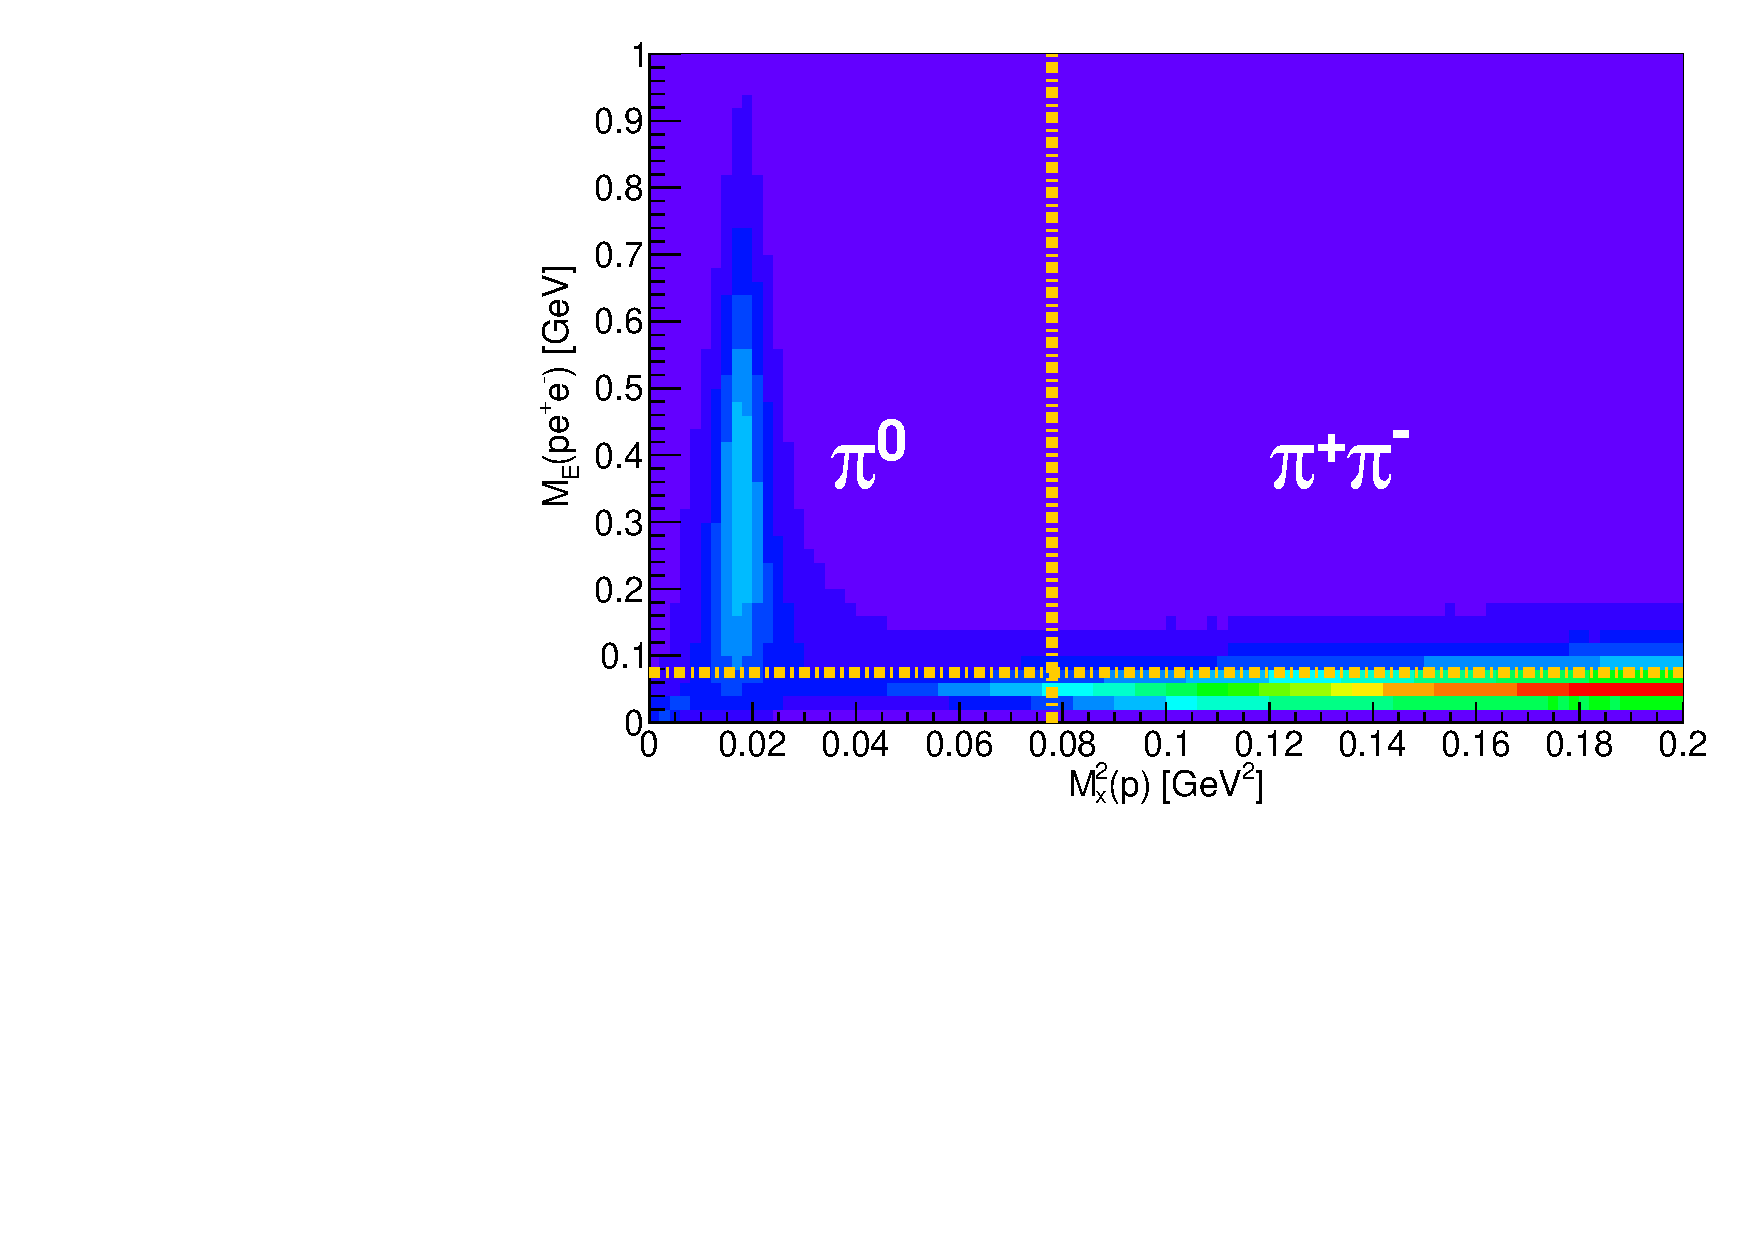
\includegraphics[height=0.4\textwidth,width=0.5\textwidth]{ME_vs_mxpcompare.pdf} \label{fig:beforecut}\hfill
		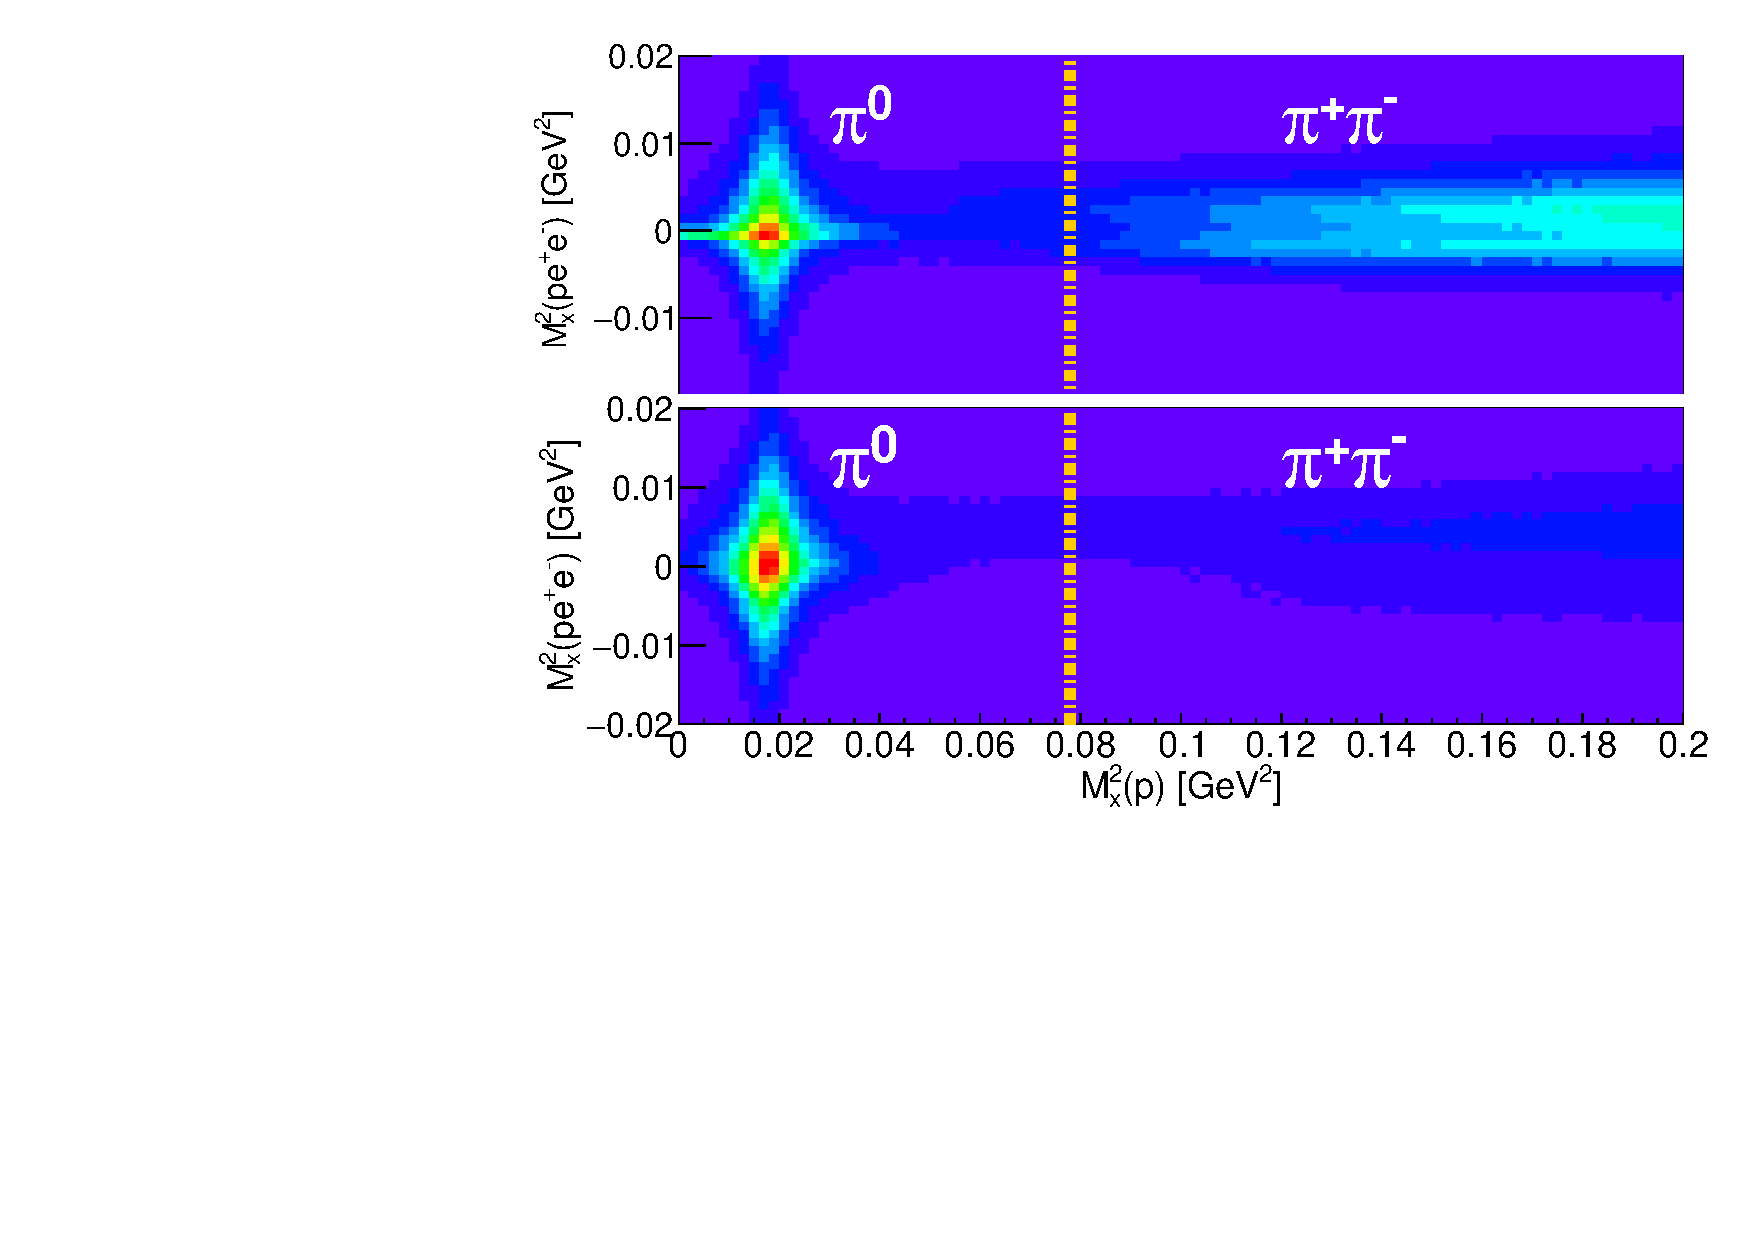
\includegraphics[height=0.4\textwidth,width=0.5\textwidth]{mm2_vs_mxp_compare.pdf}
		\label{fig:aftercut}}	
	\caption{(Color online)(left panel)$\mathrm{M_x^2(p)}$ vs. $\mathrm{M_E(pe^+e^-)}$. (Right panel)$\mathrm{M_x^2(p)}$ vs. $\mathrm{M_x^2(pe^+e^-)}$;(right-top panel)before applying the $\mathrm{M_E(pe^+e^-)} <$ 75~MeV condition, (tight-bottom panel) after applying the $\mathrm{M_E(pe^+e^-)} <$ 75~MeV condition. The horizontal orange dashed-dotted line depicted on the left-bottom panel illustrates the 75~MeV threshold used in this analysis. The vertical orange dashed-dotted line depicts boundary of single \pizT to $\pi^+\pi^-$  production.	
	}\label{fig:sys}		
\end{figure*}

Overall, angular independent systematic uncertainty varies 
between 9\% and 12\% as a function of photon energy. The 
individual contributions came from particle efficiency, 
sector-to-sector efficiency, flux determination, missing energy cut, 
4-C, 2-C, and 1-C pull probability, target length, branching 
ratio, fiducial cut, and z-vertex cut.

The missing mass of proton for events 
with $pe^+e^-(\gamma)$ in final state shown in 
Fig.~\ref{fig:pi0_peak}. The selected strategy of the analysis
of $g12$ data allowed to have negligible background vs., for 
instance, $g1c$ results published recently~\cite{du07}.  The 
fit (shown by red solid line) is performed with the Crystal Ball function~\cite{Ball1,Ball2}(shown by blue-dashed line) for the signal, plus 3rd 
order polynomial function (shown by cyan-dashed line) for the background. The fit results in $M_{\pi^0}^2$ = 
0.0179~GeV$^2$ and the Gaussian $\sigma$=0.0049~GeV$^2$. To select \pizT events, a 3.5$\sigma$ cut is placed on the fit function (shown in vertical red-dashed lines), which results in a $\frac{\mathrm{signal}}{\mathrm{signal + background}} = 98.6\%$.
%--------------------------------------------------
\begin{figure}[htb!]
\centerline{
        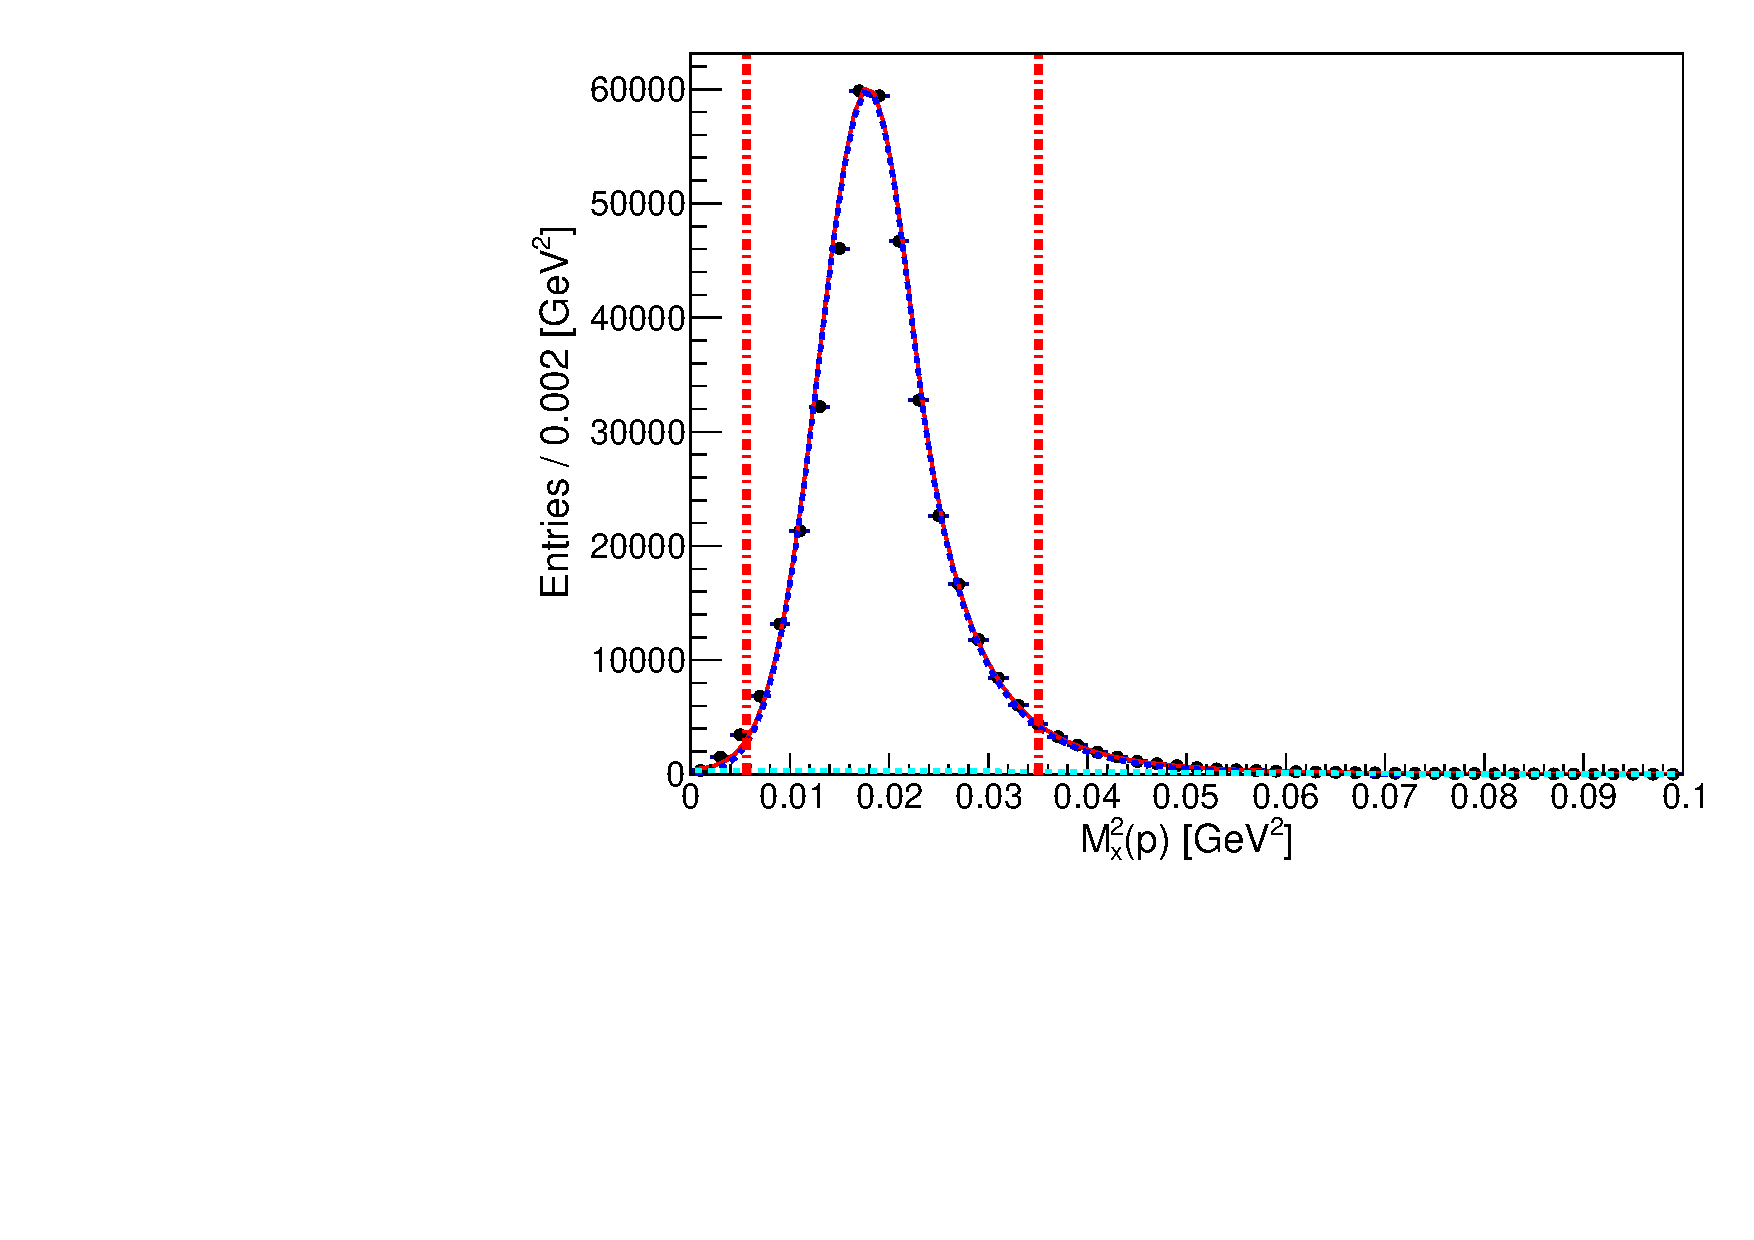
\includegraphics[height=0.4\textwidth,width=0.5\textwidth]{G12_Pi0_thesis.pdf}}

%%% trying .pdf instead of .eps
        \caption {(Color online) Peak of $\pi^0$ in the missing
                mass of proton for events with $pe^+e^-(\gamma)$
                in final state. The red-solid line, on-top of blue-dashed line depicts the fit function and signal function respectively. The cyan-dashed line, seen towards the bottom, if the result of the background fit function. The vertical red dashed-dotted line depicts boundary of a 3.5$\sigma$ cut placed on these \pizT events.} \label{fig:pi0_peak}
\end{figure}
%-----------------------------------------------------
%\textbf{Results:} 

The new CLAS high statistical cross sections, 
obtained here, for $\gamma p\to\pi^0p$ are compared in 
Figs.~\ref{fig:scaling} and \ref{fig:t_data} with previous 
data from tagged JLab CLAS $g1c$ measurements~\cite{du07}, and 
bremsstrahlung DESY, Cambridge Electron Accelerator (CEA), and 
SLAC, and Electron Synchrotron at Cornell Univ.
experiments~\cite{brem}. The overall agreement is good, 
particularly  with the tagged CLAS $g1c$ data.
%----------------------------------------------------
\begin{figure*}[htb!]
\centerline{
	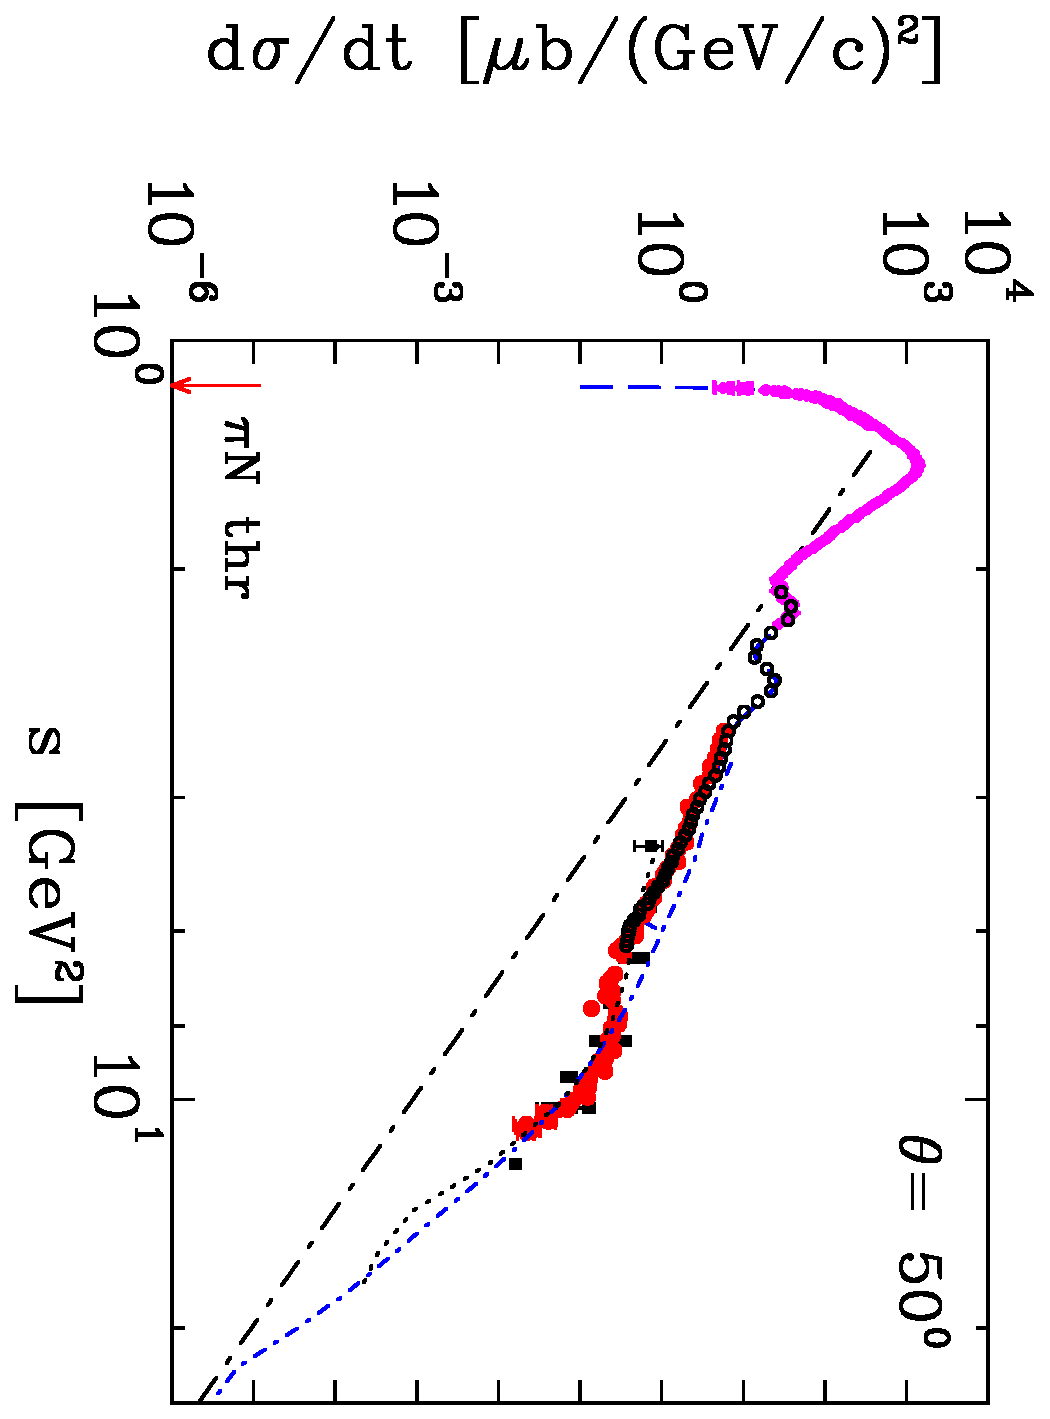
\includegraphics[height=0.4\textwidth, angle=90]{scale50.eps}\hfill
	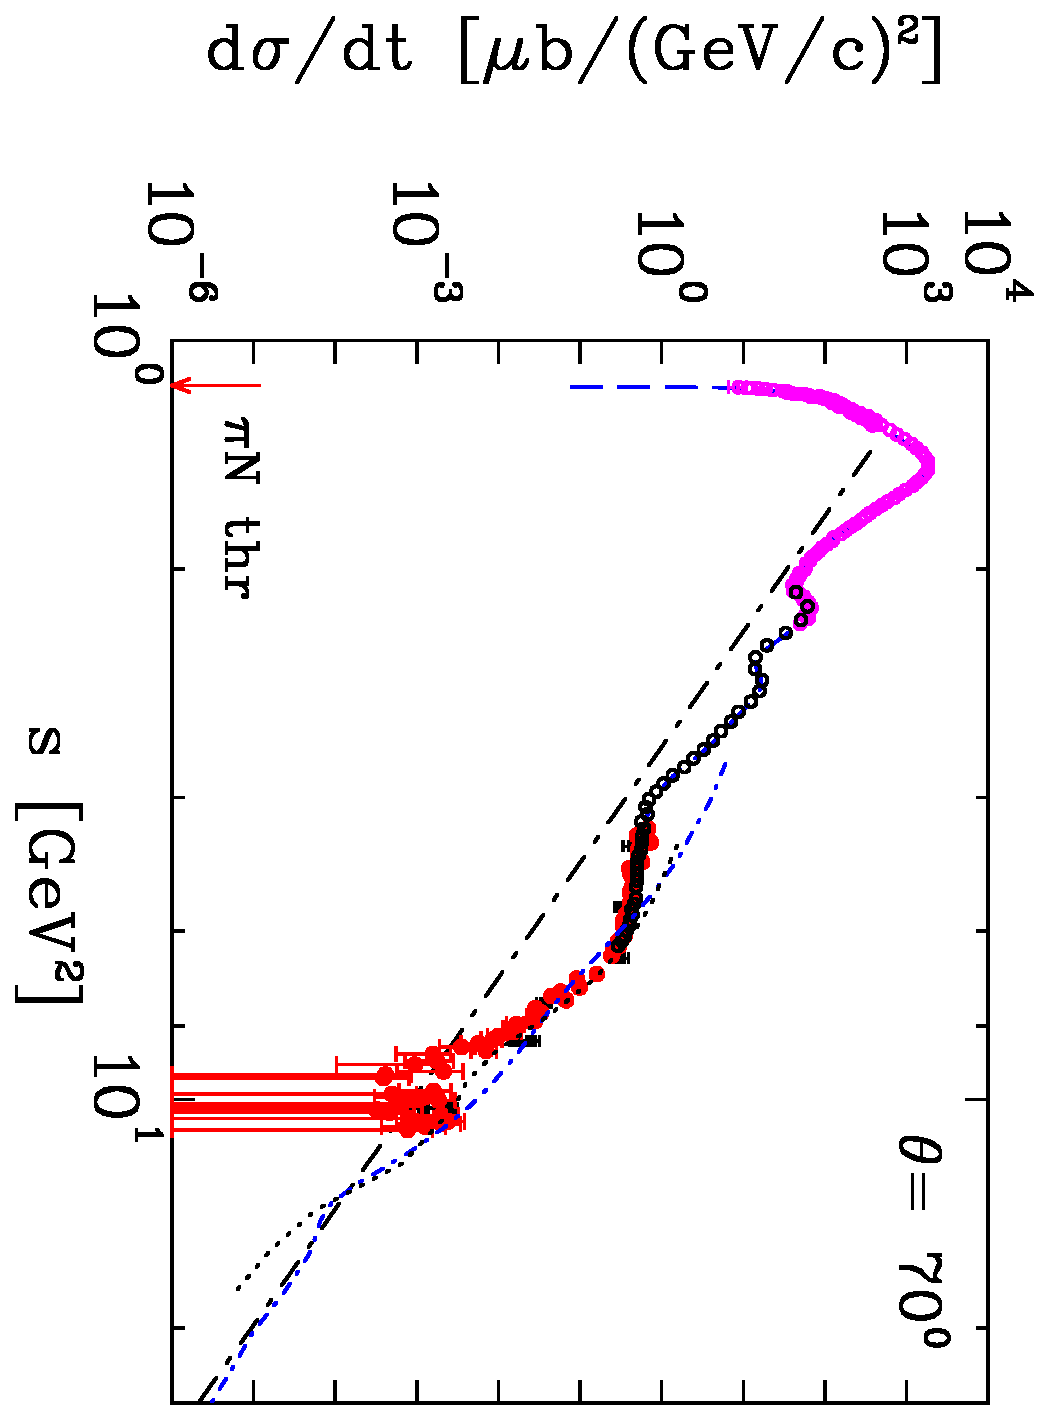
\includegraphics[height=0.4\textwidth, angle=90]{scale70.eps}}
\centerline{
        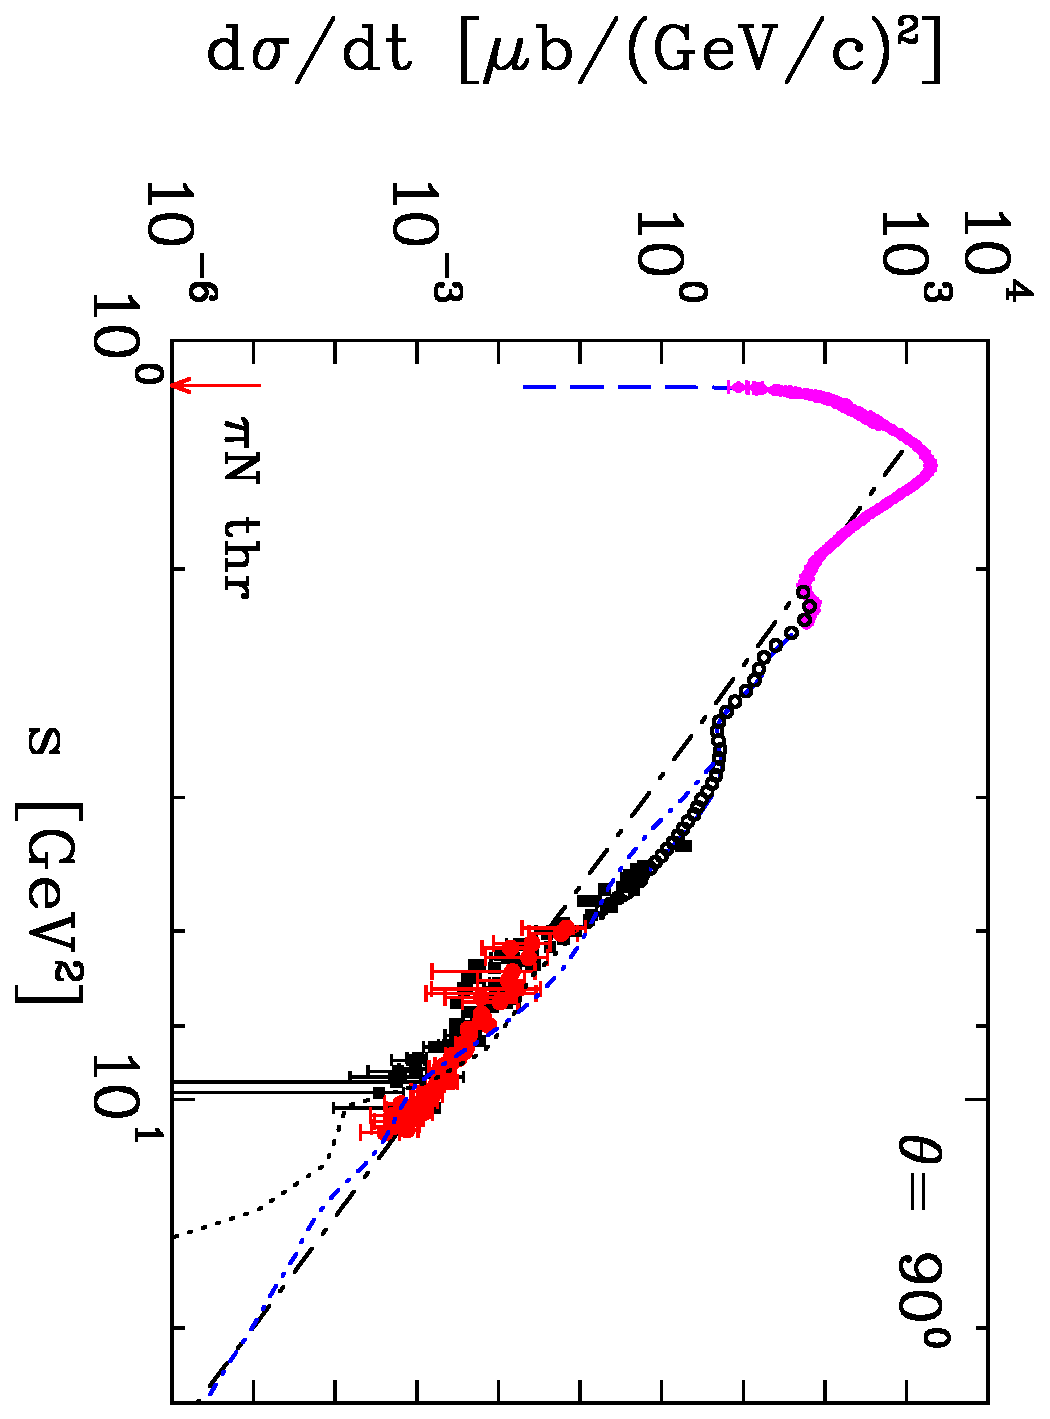
\includegraphics[height=0.4\textwidth, angle=90]{scale90.eps}\hfill
        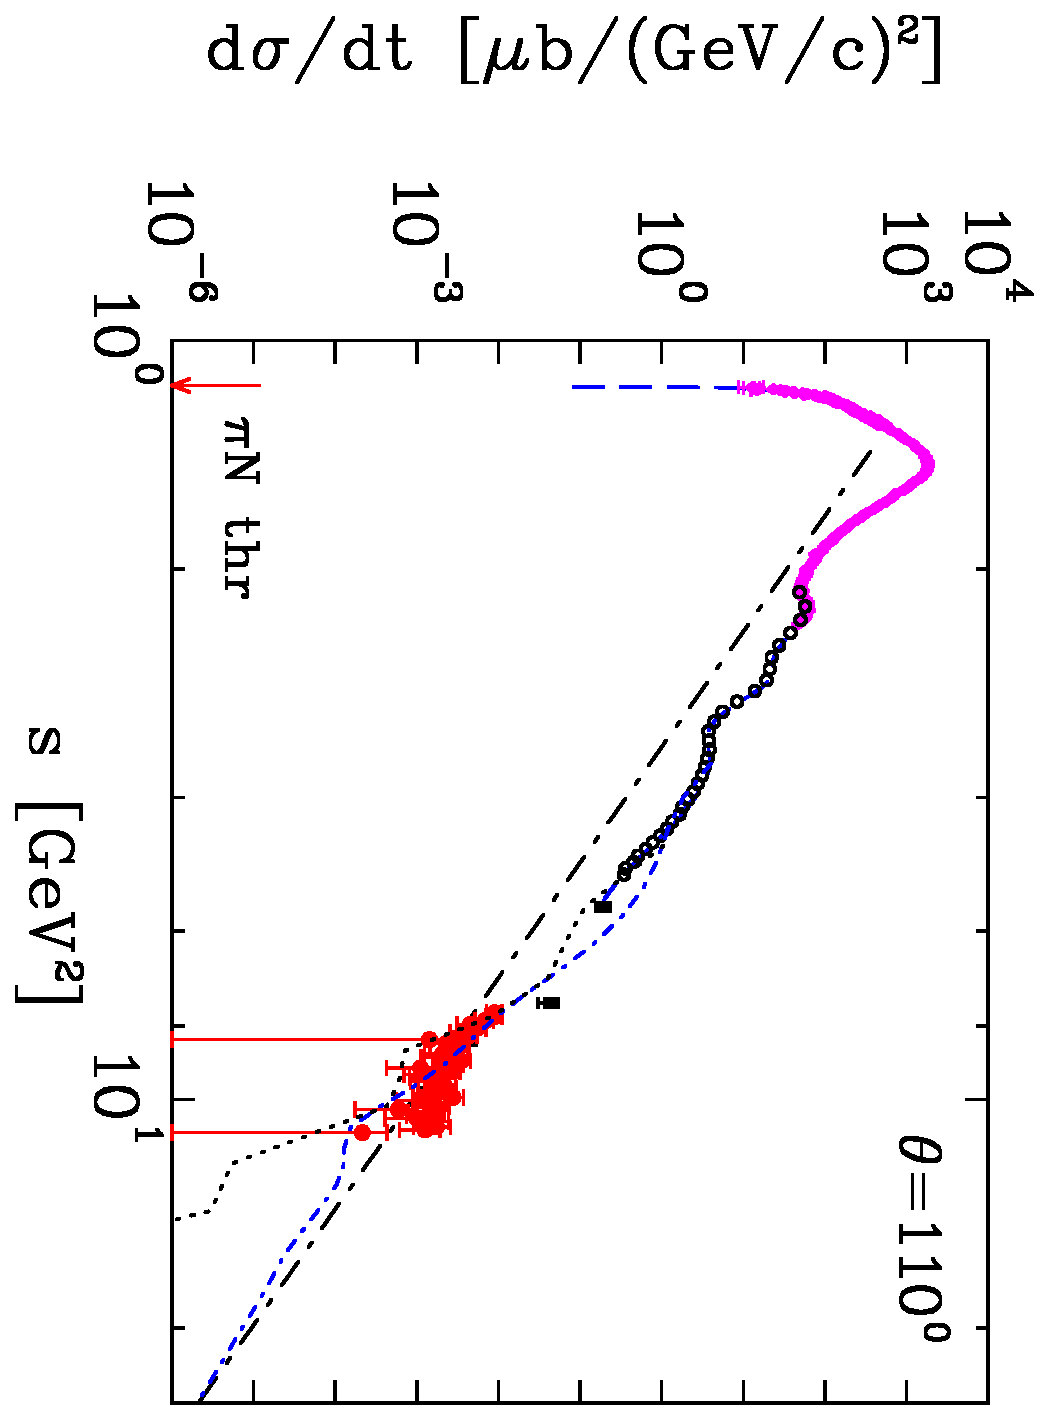
\includegraphics[height=0.4\textwidth, angle=90]{scale110.eps}}

        \caption {(Color online) Differential cross section of 
		$\gamma p\to\pi^0p$ d$\sigma$/dt(s) at 
		50$^\circ$, 70$^\circ$, 90$^\circ$, and 
		110$^\circ$ in c.m. as a function of c.m. 
		energy squared, $s$. The red filled circles are 
		results from the current analysis of the CLAS 
		Collaboration $g12$ data. The recent tagged data 
		are from CLAS $g1c$~\protect\cite{du07} (black 
		open circles) and A2 at MAMI 
		Collaboration~\protect\cite{mami} (magenta open 
		diamonds with crosses). While black open filled 
		squares are data from old bremsstrahlung
		measurements above E = 2~GeV~\protect\cite{brem}. 
		The plotted points from previously published 
		experimental data within $\Delta\theta =
		\pm$2$^\circ$ of pion c.m. production angle, 
		$\theta$.  Plotted uncertainties are statistical.  
		The blue dashed line corresponds to the SAID PWA 
		DU13 solution (no new CLAS data are in the 
		fit)~\protect\cite{du13}.  Black dot-dashed lines 
		are plotted as the best fit result for
		90$^\circ$ case. Pion production threshold shown 
		as a vertical red arrow. Regge 
		results~\protect\cite{Goldstein,Laget} are given 
		by black dotted and blue short dash-dotted, 
		respectively.} \label{fig:scaling}
\end{figure*}
%-----------------------------------------------------

%-----------------------------------------------------
\begin{figure*}[htb!]
\centerline{
        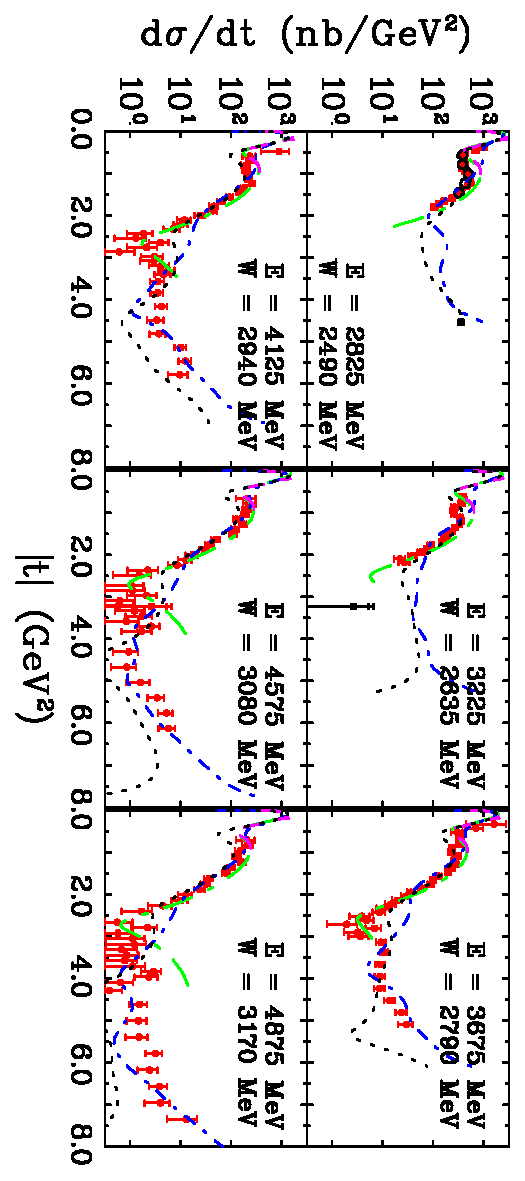
\includegraphics[width=3in, angle=90]{dsdt.eps}}

        \caption {(Color online) Samples of the $\pi^0$ 
		photoproduction cross section, $d\sigma/dt(|t|)$, 
		off the proton versus $|t|$ above "resonance" 
		regime.  Tagged experimental data are from the 
		current CLAS $g12$ (red filled circles) and CLAS 
		$g1c$~\protect\cite{du07} (black open circles). 
		The plotted points from previously published 
		bremsstrahlung experimental data above E = 
		2~GeV~\protect\cite{brem} (black filled squares) 
		are those data points within $\Delta E = \pm$3~MeV 
		of photon energy in laboratory system indicated on 
		each panel. Plotted uncertainties are statistical.  
		Regge results~\protect\cite{Goldstein,Laget,
		Mathieu,Donnachie} are given by black dotted, 
		blue short dash-dotted, green long dash-dotted, 
		and magenta long dashed lines, respectively.} 
		\label{fig:t_data}
\end{figure*}
%-----------------------------------------------------
%\FloatBarrier
%-----------------------------------------------------
%\textbf{Scaling:}  
At higher energies (above $s\sim$ 6~GeV$^2$) and large c.m. angles 
($\theta\geq$ 90$^\circ$) in c.m., the results are consistent 
with the $s^{-7}$ scaling, at fixed $t/s$, as expected from the quark counting 
rule~\cite{Stan}. The black dash-dotted line at 90$^\circ$ 
(Fig.~\ref{fig:scaling}) is a result of the fit of new CLAS 
$g12$ data only, performed with a power function $\sim s^{-n}$, 
leading to n = 6.89$\pm$0.26.  Oscillations observed at 
50$^\circ$ and 70$^\circ$ up to s$\sim$10~GeV$^2$ indicate
that the quark counting rule requires higher energies and 
higher $|t|$ before it can provide a valid description.

%-----------------------------------------------------
%\textbf{Comparison to Phenomenological Models:} 
In Figs.~\ref{fig:t_data} and \ref{fig:kroll}, the 
$d\sigma/dt(|t|)$ values, where $t$ is the squared four-momentum 
transfer, are shown along with predictions from Regge 
pole and cut~\cite{Goldstein,Laget,Mathieu,Donnachie} models and the
handbag~\cite{Kroll} model. 

Below $|t|\sim$0.6~GeV$^2$ there is a small difference between different Regge 
approaches.  Overall, the Regge approximation becomes less 
relevant below E = 3~GeV (Fig.~\ref{fig:t_data}).  CLAS data 
make this statement more apparent.  Note that some small 
structures start to appear around $|t| = 
0.3-0.6$~GeV$^2$~($\cos\theta = 0.6-0.8$) below E = 4~GeV.  The dip 
around $|t| = 0.9-1.2$~GeV$^2$ ($\cos\theta = 0.2-0.4$) (moving 
with energy) agrees with the presented CLAS data.  This is surprising.  
There was no evidence found before (with the actual data) for 
this dip. Note that the Regge amplitudes imposes non negligible 
constraints for the "resonance" region.  Our data show two more 
visible dips above E = 4~GeV and around $|t|\sim$3~GeV$^2$ and 
$|t|\sim$5~GeV$^2$. The Regge model predicts ``nonsense, wrong 
signature zeroes" where the Regge trajectories cross negative 
even integers. For the dominant vector meson Regge poles, these 
dips should appear at approximately $-t=0.6, \, 3.0, \, 
5.0$~GeV$^2$,  which agrees with the data.  That is why 
it is also important to study the high energy region, above 
"resonance" regime.

The Reggeon trajectories and cancellation of singularities in $|t|$ 
gives rise to zeroes in the various combinations of helicity 
amplitudes. These are seen as dips in the cross sections. Dips that 
occur for one Regge trajectory are filled in by the contributions 
from other, distinct trajectories. That is, the zeroes for the 
$\rho^0, \, \omega$ trajectories occur at different values of $|t|$ 
than those of the $b_1^0, \, h_1$ trajectories. Nevertheless, 
because the two sets have opposite naturality (parity $(-1)^J$ or 
$(-1)^{J+1}$), there are combinations of helicity amplitudes that 
will separate into ``natural" and ``unnatural" parity.  Those would 
have zeroes separately. Since zeroes are not observed, but dips 
are, a mechanism for producing those dips is provided by final 
state interactions which correspond to Regge cuts (for an 
alternative Regge cut model see, for instance, Ref.~\cite{Laget}). 
Those were implemented in an eikonal formalism. It was expected 
that the appropriate range of $|t|$ was roughly $0 < |t| 
<$1.3~GeV$^2$. Since these data cover that full range of $|t|$, it 
is interesting to see how the old model, for instance~\cite{Goldstein}, 
fares in an enlarged range. Remarkably, with a lowering of the 
original Pomeron strength, %(by eyeball)
the model agrees with the data 
fairly well up to the $90^\circ$.  The description of the $\pi^0$ 
photoproduction cross sections at largest $|t|$ requires some
improvement of the Regge model probably by including u-channel 
exchange.

Simultaneously, Fig.~\ref{fig:kroll} shows that the new CLAS data 
%disesteem 
are orders of magnitude higher than 
the handbag model for $\pi^0$ photoproduction below 
$s$ = 11~GeV$^2$.

%------------------------------------------------------
\begin{figure}[htb!]
\centerline{
        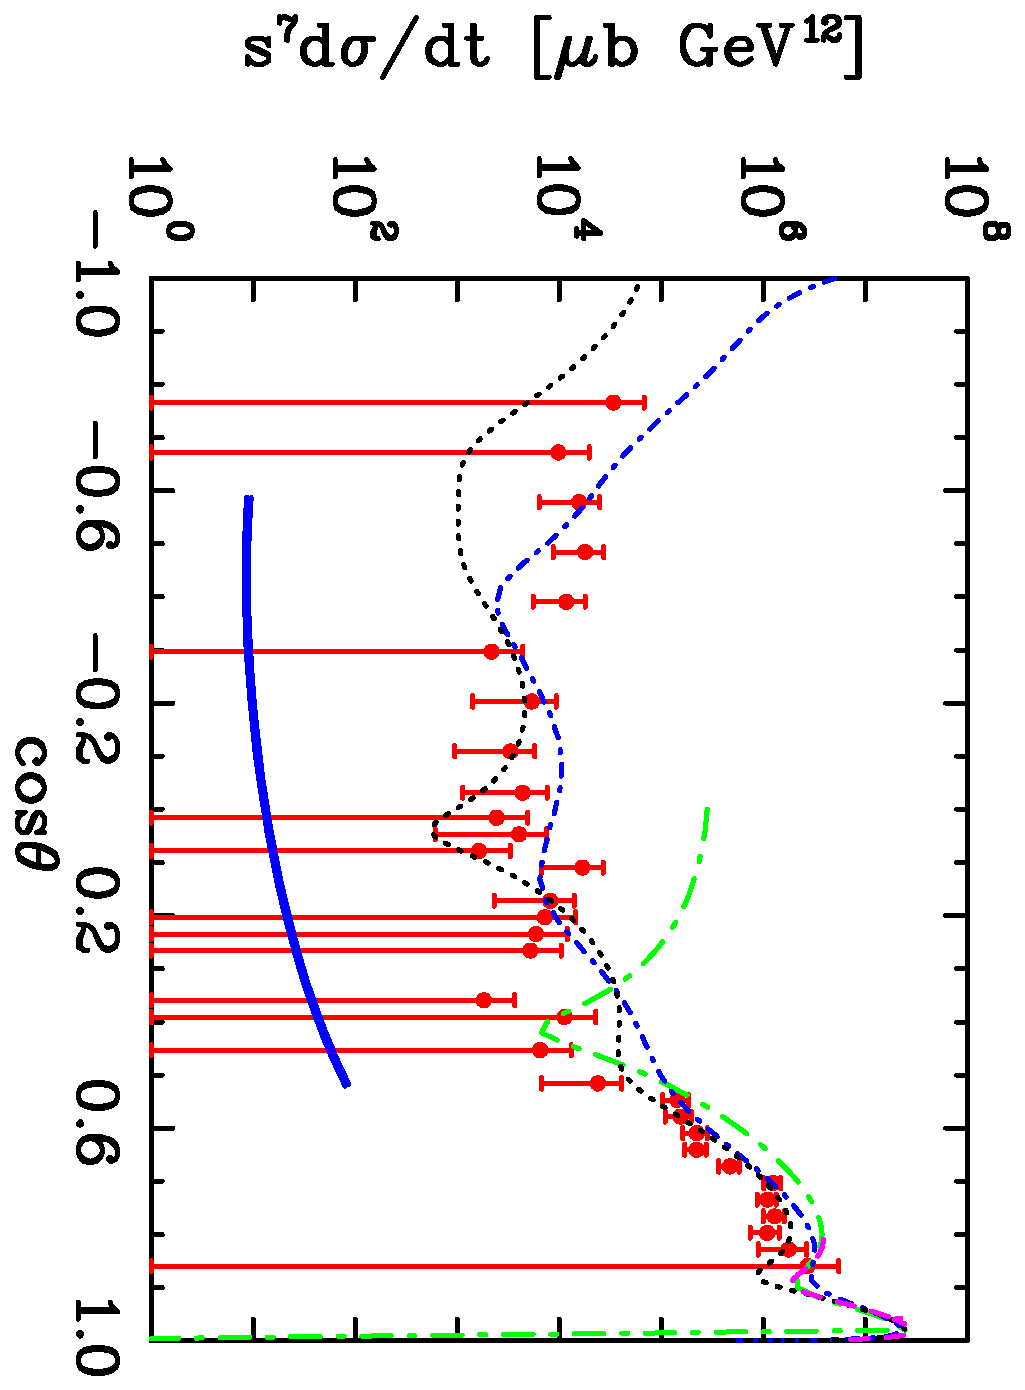
\includegraphics[width=2.5in, angle=90]{kroll.eps}}

        \caption {(Color online) Differential cross section 
		of $\pi^0$ photoproduction. CLAS experimental 
		data at $s$ = 11~GeV$^2$ are from the 
		current $g12$ experiment (red filled circles).  
		The theoretical curves a given for Regge 
		fits are the same as in 
		Fig.~\protect\ref{fig:t_data} and handbag model 
		by Kroll~\protect\textit{et 
		al.}~\protect\cite{Kroll} at $s$ = 10~GeV$^2$ 
		(blue double solid line).} 
		\label{fig:kroll}
\end{figure}
%-----------------------------------------------------
%\FloatBarrier
%-----------------------------------------------------
%\textbf{Conclusions:} 
A significant increase in the 
comprehensiveness of the database for observables in the meson 
photoproduction process is critical to reaching definitive 
knowledge about QCD-based models of the nucleon. Studies that 
cover a broad range of c.m. energy $\sqrt{s}$ are particularly 
helpful in sorting out the phenomenology.

Through the experiments described above, an extensive and
precise data set (2030 data points) on the cross section for 
$\pi^0$ photoproduction from the proton has been obtained over 
the range of $1.81~\leq W\leq 3.33$~GeV. A novel approach based 
on the use of the Dalitz decay mode was employed for extracting the 
cross sections from the experimental data. Measurements are 
performed in the reaction $\gamma p\to pe^+e^-X(\gamma)$ using a 
tagged photon beam spanning the energy interval covered by 
"resonance" and "Regge" regimes.

The measurements obtained here have been compared to
existing data. The overall agreement is good, while the 
data provided here quadripleted the world bremsstrahlung 
database above E = 2~GeV, more precise than previous 
measurements, and cover the reported energies with finer 
resolution.  By comparing this new and greatly expanded data 
set to the predictions of several phenomenological models, 
the present data were found to favor the Regge pole model 
and quark counting rule while disfavoring the 
handbag approach.  

%---------------------------------------------
\FloatBarrier
%\textbf{Acknowledgements:}  
We thank Stanley Brodsky, Alexander Donnachie, 
Peter Kroll, Jean-Marc Laget, Vincent Mathieu, 
and Anatoly Radyushkin for discussions of our 
measurements. We would like to acknowledge the outstanding 
efforts of the staff of the Accelerator and the Physics 
Divisions at Jefferson Lab that made the experiment possible.  
This work was supported in part by the Italian Istituto 
Nazionale di Fisica Nucleare, the French Centre National de 
la Recherche Scientifique and Commissariat \`a l'Energie 
Atomique, the United Kingdom's Science and Technology 
Facilities Council (STFC), the U.S. DOE and NSF, and the 
Korea Science and Engineering Foundation. The Southeastern 
Universities Research Association (SURA) operates the Thomas 
Jefferson National Accelerator Facility for the US DOE under 
contract DEAC05--84ER40150.


%-----------------------------------------------------------
\begin{thebibliography}{99}
\bibitem{Ader} J.~P.~Ader, M.~Capdeville, and Ph.~Salin, Nucl.\ 
	Phys.\ \textbf{B3}, 407 (1967).
\bibitem{Armenian} H.~K.~Armenian,  G.~R.~Goldstein, J.~P.~Rutherfoord, 
	and D.~L.~Weaver, Phys.\ Rev.\ D\ \textbf{12}, 1278 (1975).
\bibitem{Stan}S.~J.~Brodsky and G.~R.~Farrar, Phys.\ Rev.\ Lett.\
        \textbf{31}, 1153 (1973).
\bibitem{Goldstein} G.~R.~Goldstein and J.~F.~Owens~III, Phys.\ 
	Rev.\ D\ \textbf{7}, 865 (1973).
\bibitem{Laget} J.-M.~Laget, Phys.\ Rev.\ C\ \textbf{72}, 
	022202(R) (2005).
\bibitem{Mathieu} V.~Mathieu, G.~Fox, and A.~Szczepaniak, Phys.\ 
	Rev.\ D\ \textbf{92}, 074013 (2015).
\bibitem{Donnachie} A.~Donnachie and Yu.~S.~Kalashnikova, Phys.\ 
	Rev.\ C\ \textbf{93}, 025203 (2016).
\bibitem{Kroll} H.~W.~Huang and P.~Kroll, Eur.\ Phys.\ J.\ C\ 
	\textbf{17}, 423 (2000);
        H.~W.~Huang, R.~Jakob, P.~Kroll, and K.~Passek-Kumericki, 
	Eur.\ Phys.\ J.\ C\ \textbf{33}, 91 (2004);
        M.~Diehl and P.~Kroll, arXiv:1302.4604 [hep--ph].
\bibitem{HM}X.~Ji, Phys.\ Rev.\ Lett.\ \textbf{78}, 610 (1997); 
	Phys.\ Rev.\ D\ \textbf{55}, 7114 (1997); 
	A.~V.~Radyushkin, Phys.\ Lett.\ B\ \textbf{380}, 417 (1996); 
	Phys.\ Rev.\ D\ \textbf{56}, 5524 (1997); 
	D.~Muller, {\it et al.} 
\bibitem{Anderson} R.~L.~Anderson \textit{et al.}, Phys.\ Rev.\ D\
        \textbf{14}, 679 (1976).
\bibitem{Jenkins} D.~A.~Jenkins and I.~I.~Strakovsky, Phys.\ Rev.\ C\
        \textbf{52}, 3499 (1995).
\bibitem{Zhu} L.~Y.~Zhu \textit{et al.} (Jefferson Lab Hall~A
        Collaboration), Phys.\ Rev.\ Lett.\ \textbf{91}, 022003 (2003).
\bibitem{Chen} W.~Chen \textit{et al.} (CLAS Collaboration),
        Phys.\ Rev.\ Lett.\ \textbf{103}, 012301 (2009).
\bibitem{Kong} Kook-Jin~Kong, Tae~Keun~Choi, and Byung-Geel~Yu, Phys.\ 
        Rev.\ C\ \textbf{94}, 025202 (2016).
\bibitem{brem} The Durham HEP Reaction Data Databases (UK) (Durham 
	HepData): http://durpdg.dur.ac.uk/hepdata/reac.html .
\bibitem{du07} M.~Dugger \textit{et al.} (CLAS Collaboration),
        Phys.\ Rev.\ C\ \textbf{76}, 025211 (2007).
\bibitem{g12} G12 experiemental group, CLAS Technical Note, 2016.
\bibitem{Ball1} M.~J.~Oreglia, SLAC-236 UC-34d (T/E/I).  Ph.~D.~Dissertation, SLAC, 1980.
\bibitem{Ball2}T.~Skwarnicki, DESY F31-86-02, Ph.~D.~Dissertation, Inst. of Nucl. Phys. Cracow, Poland, 1986.
\bibitem{Kunkel} M.~C.~Kunkel, Ph.~D.~Dissertation, ODU, 2014.
%       https://www.jlab.org/Hall-B/general/thesis/Kunkel_thesis.pdf .
\bibitem{mami}M.~Fuchs \textit{et al.}, Phys.\ Lett.\ B\ 
	\textbf{368}, 20 (1996); 
	R.~Beck \textit{et al.}, Eur.\ Phys.\ J.\ A\ \textbf{28S1}, 
	173 (2006).
\bibitem{du13} M.~Dugger \textit{et al.} (CLAS Collaboration), 
	Phys.\ Rev.\ C\ \textbf{88}, 065203 (2013).
%\bibitem{Moskov}M.~Amarian \textit{et al.} (HERMES Collaboration), 
%AIP\ Conf.\ Proc.\ \textbf{570}, 428 (2001), Proceedings 
%of the \textit{14th International Spin Physics Symposium} 
%(SPIN 2000), Osaka, Japan, Oct. 2000, edited by K.~Hatanaka, 
%T.~Nakano, K.~Imai, and H.~Ejiri.	
\end{thebibliography}
%---------------------------------------------------------------------
\end{document}
